\documentclass[a4paper, 14pt]{article}

\usepackage[margin=3cm]{geometry}
\usepackage[utf8]{inputenc}
\usepackage[ngerman]{babel}
\usepackage[autostyle=true,german=quotes]{csquotes}
\usepackage{amsmath}
\usepackage{amssymb}
\usepackage{graphicx}
\usepackage{hyperref}
\usepackage{tikz}
\usepackage{multirow}
\usepackage{array}
\usetikzlibrary{
	calc
}

\author{Paul Brinkmeier}
\title{Cheatsheet für Einführung in Rechnernetze}

\begin{document}
	\maketitle
	\newpage
	\tableofcontents
	\newpage

	\raggedright

	\section{Grundlegende Grundlagen}

	\paragraph{Rechnernetz}

	Ein Rechnernetz besteht aus Komponenten und Übertragungsmedien, die diese Komponenten miteinander verbinden.
	Übertragungsmedien realisieren die sogenannten Kommunikationslinks (Übertragungsstrecken) zwischen Komponenten.

	Komponenten sind beispielsweise Computer, Smartphones, Kühlschränke, Router.

	Medien sind beispielsweise Koaxialkabel, Kupferkabel, Glasfaser, Funk.

	\paragraph{Endsystem}

	Endsysteme (Hosts) führen verteilte Anwendungen aus.
	Diese benötigen ein Rechnernetz zur Kommunikation zwischen Anwendungsinstanzen.
	Beispiele für verteilte Anwendungen und Endsysteme: WhatsApp auf Smartphone, E-Mail auf Server, etc.

	\paragraph{Zwischensystem}

	Zwischensysteme leiten Daten im Netz weiter und führen i.d.R. keine verteilten Anwendungen aus.
	Beispiele für Zwischensysteme: Router, Switch.

	\paragraph{(Kommunikations-)Protokoll}

	Protokolle definieren Regeln und Formate für die Kommunikation zwischen zwei oder mehreren Computern sowie die beim Senden und Empfangen von Daten bzw. bei Ereignissen auszuführenden Aktionen.

	\paragraph{(Daten-)Pakete}

	Die von Anwendungen zu sendenden Daten können in kleinere Teile gegliedert werden.
	Diese werden als (Daten-)Pakete bezeichnet.
	Pakete sind aufgebaut aus Metadaten und Nutzdaten.
	Metadaten sind nur für die Abwicklung des Protokolls erforderlich; Nutzdaten sind die eigentlichen für die Anwendung wichtigen Daten.
	I.d.R. werden Pakete in Rechnernetzen unabhängig voneinander bearbeitet.

	\paragraph{Datenrate (Übertragungsrate)}

	Die Datenrate bezeichnet die Geschwindigkeit, mit der Daten zwischen zwei Komponenten übertragen wird.
	Sie wird in bit/s gemessen.
	Größenordnungen: K, M, G, T, etc. \emph{nicht} Ki, Mi, Gi, Ti!

	\subsection{Netzkern und Netzrand}

	\paragraph{Netzkern}

	Der Netzkern besteht aus den Netzen untereinander verbunderer Internet Service Provider (ISPs).
	Er beschäftigt sich vor allem mit der Weiterleitung von Paketen.
	Der Netzkern ist sozusagen das \enquote{Betriebssystem} des Internets.

	\paragraph{Netzrand}

	Der Netzrand besteht aus den Netzen von Endandwendern, bspw. Heimnetze, Firmennetze und Datenzentren.
	Er beherbergt die \enquote{Anwendungen} des Internets.

	\subsection{\enquote{Provider} im Internet}

	\paragraph{Internet-Service-Provider (ISP)}

	ISPs binden Konsumenten an das Internet an.
	Dazu gehören oft tausende Kunden und auch Unternehmen.
	Bspw. Unitymedia, Telekom, 1\&1.

	Verschiedene Größenordnungen: Tier-1-ISP, Regionaler ISP, Zugangs-ISP.

	\subparagraph{Warum hierarchisch?}

	Vernetzung aller $n$ Zugangs-ISPs Verbindungen $\in O(n^2)$ $\leadsto$ skaliert nicht.

	\paragraph{Internet-Exchange-Point (IXP)}

	IXPs sorgen für Datenaustausch zwischen größeren ISPs.
	Es gibt weltweit ca. 400 IXPs.

	\paragraph{Content-Provider}

	Content-Provider erzeugen und stellen Inhalte bereit.
	Sie wollen diese so nah wie möglich an den Netzrand ($\leadsto$ zu den Kunden) bringen.
	Bspw. Google, Netflix, Amazon.

	\subsection{Modellierung}

	\paragraph{Modell}

	Ein Modell ist ein vereinfachtes Abbild der Wirklichkeit.
	Man setzt Modelle ein, um die wesentlichen Aspekte eines Systems darzustellen.
	Die innere Struktur des Systems wird abstrahiert; man modelliert die Interaktion mit dem System (Black-Box).

	\subsubsection{Grundmodell der Kommunikation}

	\begin{itemize}
		\item Sender und Empfänger (je einer oder mehrere).
		\item Abstraktes Medium.
	\end{itemize}

	\paragraph{Abstraktes Medium}
	
	Das Medium verbindet Sender und Empfänger über eine räumliche Distanz.
	Es stellt damit einen (Kommunikations-)Dienst zur Verfügung.
	Den Übergang von Sender/Empfänger zum Medium nennt man Schnittstelle.

	Ein abstraktes Medium trifft keinerlei Aussage über seine konkrete (physische) Umsetzung.

	\subsubsection{Dienstesicht}

	\paragraph{Dienstesicht}

	Betrachtung eines Rechnernetzes als Black-Box.
	Das RN erbringt einen Dienst für seine Nutzer.

	Das RN entspricht hier dem abstrakten Medium.

	\paragraph{Dienst}

	Ein Dienst bündelt zusammengehörige Funktionen und stellt diese einem Nutzer (Dienstnehmer) zur Verfügung.
	Einzelen Teile eines Dienstes können unabhängig voneinander in Anspruch genommen werden.

	Ein \emph{Dienstzugangspunkt} (Service Access Point, SAP) stellt die Schnittstelle zu einem Dienst dar.

	\emph{Dienstnehmer} nehmen eine Dienst in Anspruch.

	\emph{Dienstgeber} (Diensterbringer) stellen einen Dienst zur Verfügung.

	\emph{Dienstprimitive} beschreiben die Interaktionen zwischen Dienstnehmer und Dienstgeber.

	Die \emph{Beschreibung eines Dienstes} reflektiert das Verhalten an den Dienstzugangspunkten zum Dienstgeber.

	\begin{figure}
		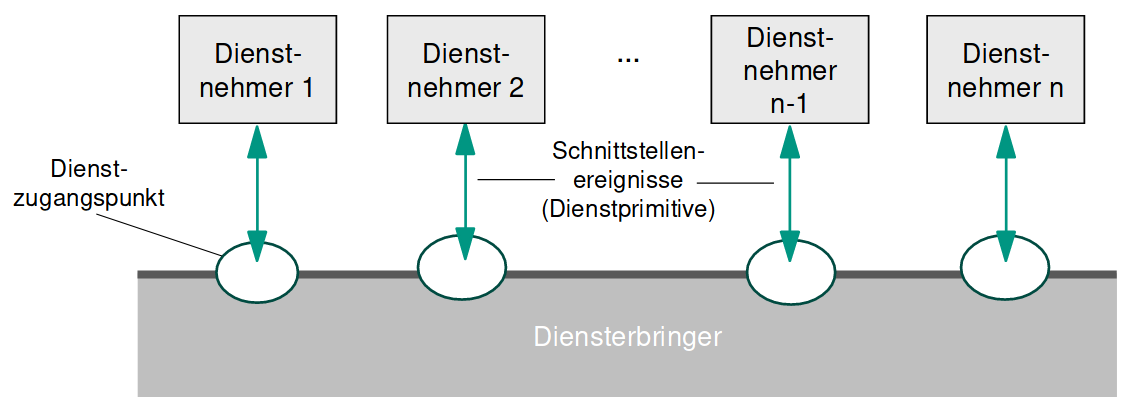
\includegraphics[width=\textwidth]{images/02-services.png}
		\caption{Dienstesicht}
	\end{figure}

	\paragraph{Dienstprimitive}

	\begin{itemize}
		\item \emph{Request} (req) --- Dienstnehmer 1 (DN1) beauftragt Dienstgeber.
		\item \emph{Indication} (ind) --- Dienstgeber benachrichtigt Dienstnehmer 2 (DN2) über Auftrag.
		\item \emph{Response} (res) --- DN2 beantwortet Auftrag.
		\item \emph{Confirmation} (cnd) --- Dienstgeber benachrichtigt DN1 über Abschluss.
	\end{itemize}

	\begin{figure}
		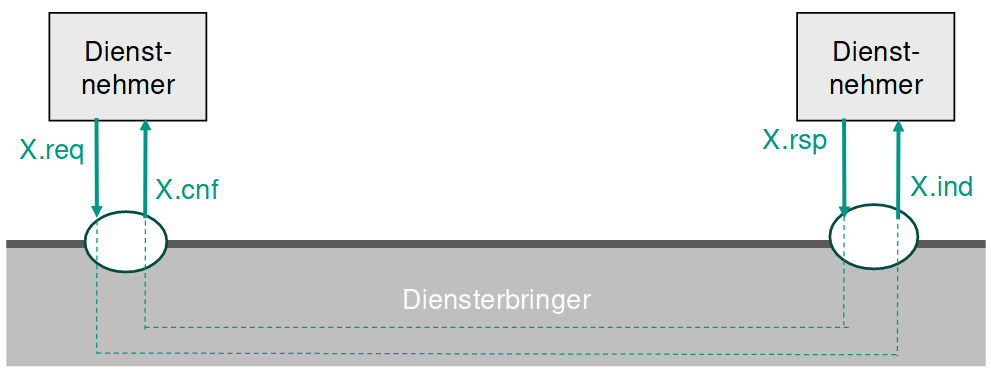
\includegraphics[width=\textwidth]{images/02-primitives.png}
		\caption{Dienstprimitive}
	\end{figure}

	\paragraph{Formen von Diensten}

	\begin{itemize}
		\item Unbestätigter Dienst --- Request (DN1), Indication (DN2).
		\item Bestätigter Dienst --- Request (DN1), Indication (DN2), Response (DN2), Confirmation (DN1).
	\end{itemize}

	\begin{figure}
		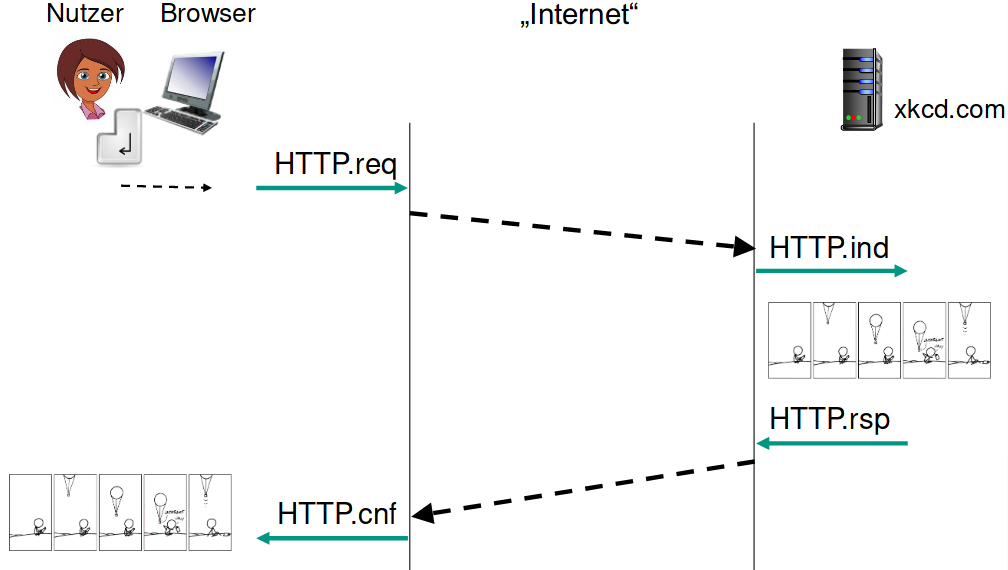
\includegraphics[width=\textwidth]{images/02-http-example.png}
		\caption{Beispiel für einen bestätigten Dienst: HTTP}
	\end{figure}

	\subsection{Zuverlässiger Dienst}

	\paragraph{Zuverlässiger Dienst}

	Bei einem zuverlässigen Dienst gilt am Dienstzugangspunkt des Empfängers folgendes:

	\begin{itemize}
		\item Alle empfangenen Daten sind korrekt.
		\item Alle vom Sender zu empfangenden Daten werden vollständig und in der richtigen Reiehnfolge empfangen.
		\item Es werden keine Duplikate empfangen.
		\item Es werden keine Phantom-Daten empfangen.
	\end{itemize}

	\textbf{Merke}: Zuverlässiger Dienst (ZD) $\neq$ Bestätigter Dienst (BD).
	Es gilt eher BD $\subset$ ZD.
	Bestätigungen sind nur \enquote{ein Baustein} zuverlässiger Dienste.

	\subsection{Schichten}

	\paragraph{Schicht}

	Eine Schicht bündelt zusammengehörige Funktionalitäten, die sich von denen anderer Schichten unterscheiden.
	Schichten sind hierarchisch angeordnet.
	An ihrer Schnittstelle stellt eine Schicht Dienste für die nächst-\enquote{höhere} Schicht bereit und nutzt Dienste der nächst-\enquote{unteren} Schicht.
	Die technische Umsetzung einer Schicht ist an dieser Schnittstelle nicht sichtbar.
	Zur Erbringung ihrere Dienste nutzt eine Schicht die Dienste der darunter liegenden Schicht.

	Protokolle sind innerhalb einer Schicht lokalisiert.

	\begin{figure}
		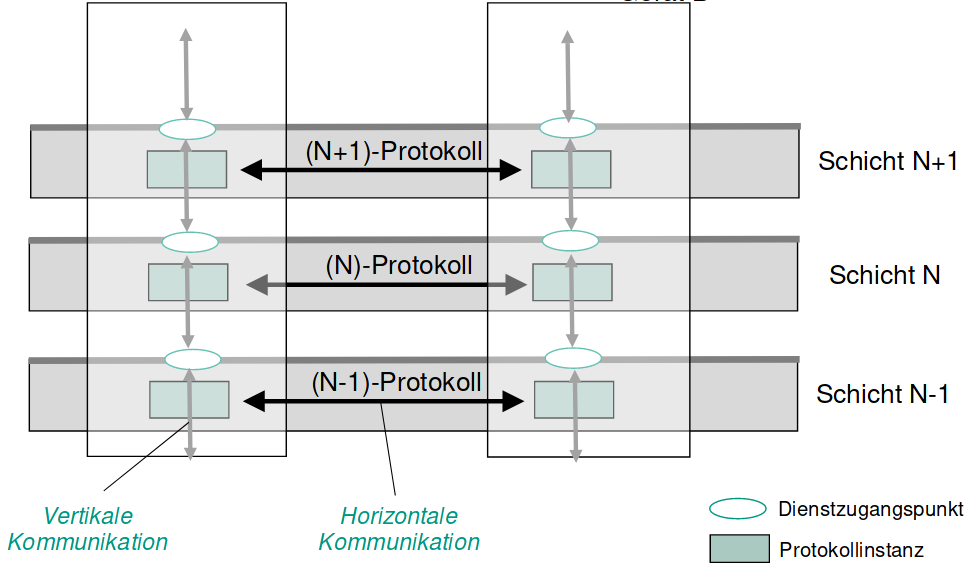
\includegraphics[width=\textwidth]{images/02-layers.png}
		\caption{Protokolle, Dienste, Schichten}
	\end{figure}

	\paragraph{Horizontale Kommunikation}

	Horizontale Kommunikation findet innerhalb einer Schicht zwischen Sender und Empfänger statt.
	Die Protokollinstanzen der Schicht (auf den jeweiligen Geräten) tauschen Daten untereinander aus, um den geforderten Dienst zu erbringen.

	\paragraph{Vertikale Kommunikation}

	Vertikale Kommunikation findet zwischen zwei Schichten innerhalb eines Gerätes statt.
	Protokollinstanz der Schicht $N$ nimmt Dienste der Schicht $N - 1$ in Anspruch oder reichen Daten an Schicht $N + 1$ weiter.

	\subsubsection{Fünf-Schichten-Referenzmodell}

	\begin{figure}
		\begin{center}
			\begin{tikzpicture}[
	>=latex
]
	\node(layers)[inner sep=0]{\Large \begin{tabular}{| c |}
		\hline
		Anwendungsschicht \\
		\hline
		Transportschicht \\
		\hline
		Vermittlungsschicht \\
		\hline
		Sicherungsschicht \\
		\hline
		Physische Schicht \\
		\hline
	\end{tabular}};

	\coordinate (T) at ($(layers.north east) + (1cm, 0)$);
	\coordinate (B) at ($(layers.south east) + (1cm, 0)$);

	\draw[->] (B) -- (T);

	\node[anchor=west] at (T) {Abstraktion hoch};
	\node[anchor=west] at (B) {Abstraktion niedrig};
\end{tikzpicture}

		\end{center}
		\caption{Referenzmodell mit fünf Schichten}
	\end{figure}

	\paragraph{Physische Schicht}

	Zwei direkt über ein Übertragungsmedium beschränkter Länge verbundene Geräte können unstrukturierte Bitfolgen austauschen.
	Eigenschaften dieser Schicht sind:

	\begin{itemize}
		\item Stellt unzuverlässigen Dienst für (Sicherungsschicht) bereit.
		\item Bits werden nicht gepuffert.
		\item Stark Hardwareabhängig (\enquote{LAN-Kabel}, Glasfaser, WLAN, etc.).
		\item Bei der Übertragung können Störungen auftreten (Paradebeispiel: WLAN).
	\end{itemize}

	\paragraph{Sicherungsschicht}

	Auf dieser Schicht werden zwischen physisch benachbarten Systemen Daten Paketweise (sog. \emph{Rahmen}) übertragen.
	Eigenschaften dieser Schicht sind:

	\begin{itemize}
		\item Ermöglicht Adressierung benachbarter Geräte.
		\item Stellt unzuverlässige und zuverlässige Dienste (Erkennung von Fehlern der physischen Schicht) bereit.
		\item Puffert Daten sowohl beim Sender als auch beim Empfänger.
		\item Abstrahiert physisches Medium.
	\end{itemize}

	\paragraph{Vermittlungsschicht}

	Diese Schicht ermöglicht den Austausch von Daten zwischen (nicht unbedingt) benachbarten Systemen über Zwischensysteme (\emph{Ende-zu-Ende}).
	Pakete nennt man hier typischerweise \emph{Datagramme}.
	Eigenschaften dieser Schicht sind:

	\begin{itemize}
		\item Universale Adressierung von Endsystemen (bspw. IP-Adressen).
		\item Stellt unzuverlässige und zuverlässige Dienste bereit.
		\item Datagramme können in Zwischensystemen gepuffert werden.
		\item Ein Datagramm wird in einem oder mehreren Rahmen der Sicherungsschicht übertragen.
	\end{itemize}

	\paragraph{Transportschicht}

	In dieser Schicht ist die Kommunikation zwischen Anwendungsprozessen auf den Endsystemen gekapselt (\emph{Nutzer-zu-Nutzer}).
	Pakete nennt man hier typischerweise \emph{Datagramme} oder \emph{Segmente}.
	Eigenschaften dieser Schicht sind:

	\begin{itemize}
		\item Adressierung von Anwendungsprozessen auf Endsystemen (\emph{Ports}).
		\item Stellt unzuverlässige (bspw. UDP) und zuverlässige (bspw. TCP) Dienste bereit.
		\item Segmente/Datagramme werden in Endsystemen gepuffert.
		\item Ein Segment/Datagramm wird in einem oder mehreren Datagrammen der Vermittlungsschicht übertragen.
	\end{itemize}

	\paragraph{Anwendungsschicht}

	Über diese Schicht tauschen Anwendungen untereinander \emph{Nachrichten} (bspw. HTTP-Response) aus.
	Je nach Anwendung werden hier zuverlässige oder unzuverlässige Dienste der Transportschicht genutzt.

	\subsubsection{TCP/IP-Referenzmodell}

	Im Internet am weitesten verbreitet (quasi alleinstehend) ist das TCP/IP-Modell.
	Dieses definiert in \href{https://tools.ietf.org/html/rfc1122}{RFC 1122} vier Schichten:

	\begin{center}
		\Large
		\begin{tabular}{| c |}
			\hline
			Anwendungsschicht \\
			\hline
			Transportschicht \\
			\hline
			Internetschicht \\
			\hline
			Netzzugang \\
			\hline
		\end{tabular}
	\end{center}

	Die Internetschicht entspricht der Vermittlungsschicht; Netzzugang kombiniert phyisische und Sicherungsschicht.
	
	\subsubsection{OSI-Referenzmodell}

	Das von der ISO standardisierte OSI-Modell (Open Systems Interconnection Model) definiert sieben Schichten:

	\begin{center}
		\Large
		\begin{tabular}{| c | c}
			\cline{1-1}
			Anwendungsschicht & \multirow{3}{*}{\normalsize Anwendungsorientierte Schichten} \\
			\cline{1-1}
			Darstellungsschicht & \\
			\cline{1-1}
			Sitzungsschicht & \\
			\hline
			Transportschicht & \multirow{4}{*}{\normalsize Transportorientierte Schichten} \\
			\cline{1-1}
			Vermittlungsschicht & \\
			\cline{1-1}
			Sicherungsschicht & \\
			\cline{1-1}
			Physische Schicht & \\
			\cline{1-1}
		\end{tabular}
	\end{center}

	\paragraph{Transportorientierte Schichten}

	Transportorientierte Schichten befassen sich mit der Übertragung von Daten zwischen Anwendungen.
	Die Semantik der übertragenen Daten spielt dabei keine Rolle.

	\paragraph{Anwendungsorientierte Schichten}

	Hier werden Anwendungsbezogene Protokolle abgewickelt.
	Die Semantik der übertragenen Daten ist wichtig.

	\begin{itemize}
		\item \emph{Sitzungsschicht} --- Bietet Nichtunterbrechbarkeit von Kommunikationsbeziehungen.
		\item \emph{Darstellungsschicht} --- Vereinheitlicht Darstellung der Daten über heterogene Systeme hinweg (bspw. Litte- vs. Big-Endian).
		\item \emph{Anwendungsschicht} --- Austausch von anwendungsspezifischen Daten.
	\end{itemize}

	\subsubsection{TCP/IP vs. OSI}

	\begin{itemize}
		\item Netzzugang $\Leftrightarrow$ OSI-Schichten 1 und 2 (physische Schicht, Sicherungsschicht).
		\item Schichten 3 und 4 (Vermittlungsschicht, Transportschicht) sind identisch.
		\item Anwendungsschicht $\Leftrightarrow$ OSI-Schichten 5 bis 7 (Sitzungs-, Darstellungs- und Anwendungsschicht).
	\end{itemize}

	Beim TCP/IP-Referenzmodell wird weniger granular zwischen den Schichten unterschieden.
	Das liegt daran, dass dieses Modell sich eher mit der Zeit aus Prototypen entwickelt hat, als dass es entworfen worden wäre.

	\section{Physische Schicht}

	\section{Sicherungsschicht}

	\section{Vermittlungsschicht}

	\section{Transportschicht}

	\section{Anwendungsschicht}

	\section{Netzssicherheit}

	\section{Klausuraufgaben}
\end{document}
